\documentclass[main.tex]{subfiles}
\begin{document}

\chapter{Results}\label{ch:results}

\section{Data Sets}
\subsection{Overview}
The data presented in this chapter were collected during a one hour measurement with both the analog and the digital setup running in parallel. A total of 4.3 million pulses from the NE213 detector were recorded by the analog setup. The digitizer saw 2.2 million pulses from the NE213 detector after the selection criteria explained in the previous chapter were applied. This large difference in counts was because the digital setup was configured to transfer each event individually. Furthermore the software \textsc{WaveDump} does not have a method for estimating livetime, so instead a livetime will be estimated by comparing with the analog setup.

In the analog setup thresholds of -25.0 mV and -94.6 mV were applied to the YAP detector and the NE213 detector, respectively. In the digital setup thresholds of -9.8 mV and -48.8 mV were applied on the YAP and the NE213 detector, respectively. Having such a low threshold on the YAP was found to decrease the signal-to-noise ratio in the ToF spectrum, so a higher threshold of -24.4\si{\milli\volt} was applied in software. Table \ref{tab:settings} presents an overview of the datasets.
\begin{table}[bh]
\begin{tabular}{|l|l|l|l|l|}
\hline
Setup   & YAP threshold(mV) & NE213 threshold(mV) & NE213 events ($\text{10}^\text{6}$) & Livetime \\ \hline
Analog  & -25.0              & -94.6                & 4.3      & 44\%             \\ \hline
Digital & -9.8/-24.4			& -48.8                & 2.2      & **             \\ \hline
\end{tabular}
\caption[Overview of the analog and digital data sets.]{Overview of the analog and digital data sets. *A threshold of \SI{24.4}{mV} was enforced offline (see text for details). **The digital setup does not have a method for determining livetime}
\label{tab:settings}
\end{table}



\subsection{Livetime and threshold alignment}
\subsubsection{Deposited energy}
The analog and the digital setup were run with different amplitude thresholds. To properly compare them a common threshold needed to be found. The analog and digital setup setups have different cable lengths to the detectors. Thus, the signals were not attenuated to the same extent. As a result the digital setup needed a significantly higher threshold in \si{mV} to accept the same events.

\begin{figure}[h!]
    \centering
        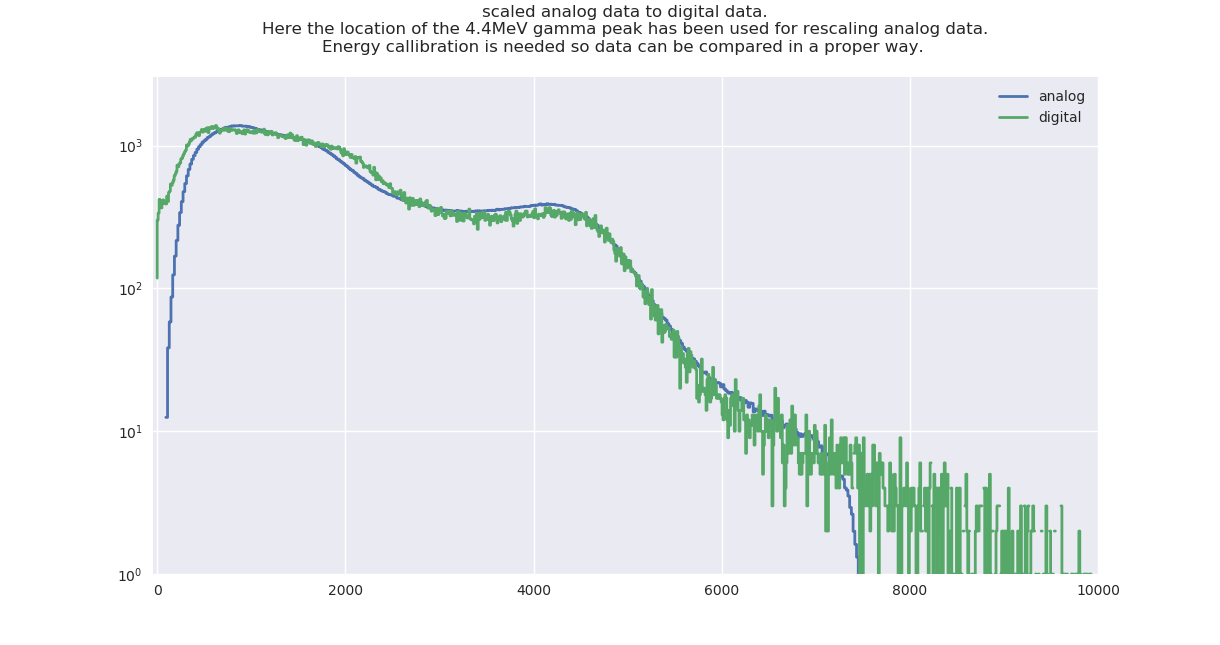
\includegraphics[width=0.7\textwidth]{CompareResults/qdc_comp.pdf}
        \caption[Comparison of analog and digital spectra from the NE213 detector]{Comparison of analog and digital spectra from the NE213 detector. Top: The red histogram is the livetime-corrected analog energy spectrum. The blue histogram is the raw digital energy spectrum and the green one is the energy spectrum from the digital setup after having been normalized to the height of the analog spectrum, and has had a pulse height threshold of 151 mV applied. Bottom: ratio of counts between livetime-corrected analog spectrum and normalized digital spectrum.}
    \label{fig:qdc_comp}
\end{figure}
Figure~\ref{fig:qdc_comp} top panel shows the energy spectra from both setups. The data from the analog setup have been livetime corrected (44\%). The blue histogram shows the raw digital spectrum, and the green histogram shows the digital spectrum after applying a higher amplitude threshold of \SI{151}{mV} and normalizing the spectrum to match the height of the livetime-corrected analog setup. This crudely fixes the livetime of the digital setup at 12\%. compared to the analog setups livetime of 44\%. The resulting spectra look more alike, although the \SI{4.44}{\MeV}$_\text{ee}$ Compton edges do not look the same. This may be because some of the high energy gamma-rays deposited energies which were outside the dynamic range of the digitizer.


Figure~\ref{fig:qdc_comp} bottom panel shows the ratio between the digital and analog spectra after livetime adjustments and threshold alignment. Ideally this ratio should be very close to 1. This is not the case. Near the \SI{4.44}{\MeV}$_\text{ee}$ Compton edge there is a bump followed by a valley. This is likely because the highest amplitude digitized pulses corresponding to the highest Compton events were clipped, causing them to be pushed to lower values of deposited energy. However a similar but smaller variation appears at \SI{2}{MeV}, which indicates that another effect might be that the digital setup has sharper Compton edges due to better energy resolution.


\subsubsection{Time-of-flight spectra}
Like the energy spectrum, the ToF spectrum is heavily influenced by the choice of amplitude threshold. Figure~\ref{fig:tof_comp} top panel shows the ToF spectra for the two setups with the initial -49 mV NE213 detector threshold on the digital setup and -94.6 mV on the analog setup. Interestingly it seems that the analog setup is cutting away the slower neutrons of this spectrum by setting a high amplitude threshold. By applying the offline NE213 detector threshold of -151 mV to the digital setup and adjusting the livetime of both setups in the same manner as before, the ToF spectrum shown in the bottom panel of Fig.~\ref{fig:tof_comp} is obtained. The neutron peaks now have roughly the same shape, which means that the amplitude cut has removed the slower neutrons.
There are more counts in the digitized ToF spectrum. This is because the YAP detector thresholds have not been aligned.
Finally, the gamma flash has a full width at half maximum of $\sim$\SI{7.7}{ns} in the analog setup and \SI{2.8}{ns} in the digital setup.

\begin{figure}[h]
    \centering
        \includegraphics[width=0.8\textwidth]{CompareResults/tof_comp.pdf}
        \caption[Analog and digital time-of-flight spectra.]{Analog and digital time-of-flight spectra. In the lower panel livetime has been taken into account and a higher threshold has been enforced on the NE213 detector signals offline.}
    \label{fig:tof_comp}
\end{figure}




\section{Analog Setup}

\subsection{Neutron Tagging}
Figure~\ref{fig:tof_a} shows the ToF spectrum recorded by the analog setup. The neutron and gamma-ray peaks are marked with arrows. In addition to these two peaks, there is an approximately flat background. This background represents uncorrelated particles triggering the TDC start and stop, which is also why negative ToF values appear.
\begin{figure}[ht]
    \centering
        \includegraphics{AnalogResults/tof.pdf}
        \caption[Time of flight spectrum, analog setup.]{The time of flight spectrum. The x-axis denotes the time of flight from source to NE213 detector. The neutron and gamma peaks have been indicated with arrows. The coincidences highlighted in red have been converted to neutron kinetic energies and are shown in the upper right insert.}
    \label{fig:tof_a}
\end{figure}

The gamma-flash peak has been shifted to be centered at \SI{3.8}{ns} (the time it takes light to travel from source to detector), but it is not entirely narrow. Since gamma-rays travel at the speed of light a narrower gamma-flash may be anticipated. The width of the gamma-flash is primarily due to the time resolution of the detectors. The detectors time resolution depends on how far the gamma-ray travels into the detector and wether or not it is scattered out of the detector before depositing its full energy. Secondary effects include attenuation in the cables, which might affect PS and thus rise time. This will in turn make the CFD less effective causing some loss in the time resolution. Furthermore, the final  digitization by the TDCs may cause some loss of resolution. Differences in flight path between gamma-rays hitting the center of the NE213 and those that hit near the edge will be less than \SI{1}{cm}, so this will not give rise to a substantial time spread. 

The neutron bump has faster neutrons at lower ToF values and slower neutrons at higher ToF values. Since the distance from source to detector is known it is possible to convert the neutron ToF into neutron kinetic energy. A range of $1.5\--7$~\si{\MeV} was used. This corresponds to a time interval of 31-\SI{68}{\ns}. The coincidences falling in this time interval have been highlighted in red in Fig.~\ref{fig:tof_a} and the corresponding energies are shown in the insert. The spectrum obtained by Scherzinger~\cite{ScherzingerPhd} (which was shown in Fig.~\ref{fig:scherzinger}) has been superimposed.

The reference spectrum was produced with the same source but a different and smaller NE213 detector. This is the reason for the large difference in count rate. Comparing with Scherzingers spectrum it appears that the slower neutrons are missing. This is likely because a too large amplitude threshold has been applied. It also appears that the energy spectrum acquired by the analog setup is shifted to the right. This may be because the higher threshold causes a higher fraction of the systems livetime to be used for high amplitude pulses. Below \SI{2.5}{MeV} the count rate in Fig.~\ref{fig:tof_a} increases. This is simply an effect of the last $\sim$\SI{20}{\ns} primarily consisting of background, and that the lowest energies covers a wider range of flight time since $E\propto \dfrac{1}{ToF^2}$.



\subsection{Pulse-Shape Discrimination}
Neutrons and gamma-rays were discriminated through the PS parameter given in Eq.~\ref{eq:ps}. The parameters $a$=120 and $b$=0 were found to linearize pulse shape as a function of energy, and gate lengths of \SI{500}{\ns} and \SI{60}{ns} were used for the LG and SG integrations respectively.

\begin{figure}[ht]
    \centering
        \includegraphics[width=\textwidth]{AnalogResults/psd_a.pdf}
        \caption[Analog PS spectrum as a function of energy deposition.]{Analog PS spectrum as a function of energy deposition. The dashed white line at 0.259 indicates the PSD cut. Structures due to the \SI{2.23}{MeV} and \SI{4.44}{MeV} gamma rays are indicated.}
        \label{fig:psd_a}
\end{figure}

PS is shown as a function of deposited energy in Fig.~\ref{fig:psd_a}. The upper band labeled neutrons consists of pulses for which the tail of the scintilation pulse resulted in a large fraction of the total charge. The lower band is made up of gamma-rays for which a smaller amount charge is in the tail of the scintillation pulse. 
This is confirmed by the presence of the compton edges corresponding to \SI{2.23}{MeV} and \SI{4.44}{MeV} gamma-rays in the lower band. The amplitude threshold of \SI{94.6}{mV} gives rise to the sloping energy threshold. This threshold has been highlighted with a red line in the figure. This is because pulses with higher PS  have more charge in tail and will contain more total charge than a pulse of equal amplitude but smaller PS.

The PS-cut value of 0.259 was found by plotting a PS histogram and fitting Gaussian functions to the neutron and gamma distribution, see~\ref{fig:fom_analog}. The quality of separation between the two distribution may be expressed as a figure of merit, FoM, defined in terms of the centers, C, of the Gaussian functions and their full width at half maximum, W.
\begin{equation}
FoM = \frac{C_n - C_\gamma}{W_n + W_\gamma}
\end{equation}
Figure~\ref{fig:fom_analog} shows histograms of the PS parameter along with the Gaussian fits used to calculate the FoM. The obtained figure of merit was 0.58, but it was found to be highly energy threshold dependent\footnote{For more information on the energy dependence of the FoM see appendix \ref{ch:appA}}.This way of parameterizing the quality of a PSD method requires that the distributions are approximately Gaussian. This assumption appears to be valid for the neutron distributions, centered at 0.3, but the gamma-ray distribution does have a tail which is not matching with the fit. The results 

%The linearization made it possible to separate the neutron and gamma-ray bands at a single PS value. The procedure by which this cut was determined will be presented in section~\ref{sec:comp}. For now it will just be noted that PS=0.259, shown as a dashed line in Fig.~\ref{fig:psd_a}, was found to provide the best separation. Seeing how the neutron and gamma-ray distributions seem to overlap at low energies this cut will likely result in misclassification. The time of flight information provides an independent parameter for distinguishing the particle species and can therefore be used to quantify the extent of the misclassification.

%---------
%---------



\begin{figure}[h!]
	    \centering
    	    \includegraphics[width=\textwidth]{CompareResults/FOM_analog.pdf}
        	\caption{Analog setup}
	    \label{fig:fom_analog} 
    \caption[Histograms of PS, with Gaussian fits for the analog setup.]{Histogram of pulseshape, with Gaussian fits to the gamma-ray and neutron distributions. The insert shows the pulse shape parameter as a function of energy, for full size version see fig~\ref{fig:psd_a}.}
\end{figure}

%--------
Figure~\ref{fig:tof_ps_a} shows pulse shape as a function of time of flight, with neutron and gamma-ray distributions highlighted. The gamma-ray and neutron distributions, marked with arrows, are somewhat overlapping, making the discrimination cut mislabel part of each distribution. Often the start and stop signal will be due to uncorrelated particles, rather than the previously discussed n-\textgamma and \textgamma-\textgamma pairs. On small timescales of a few hundred nanoseconds these events are expected to form a flat background in the time of flight spectrum, as seen in Fig.~\ref{fig:tof_a} beyond 60 ns. Since the events still represent either neutrons or gamma-rays (ignoring the occasional muon) one would expect them to be separated into two bands in Fig.~\ref{fig:tof_ps_a}. This is not the case.

\begin{figure}[ht]
    \centering
        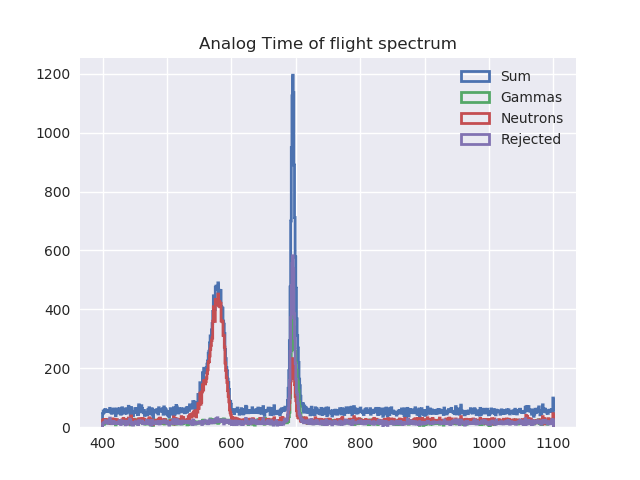
\includegraphics[width=0.8\textwidth]{AnalogResults/tof_psd.pdf}
        \caption[Heat map of pulse shape as a function of time of flight.]{Time of flight plotted against pulse shape as recorded with the analog setup. The dashed white line indicates the discrimination cut at PS=0.259. A logarithmic z-axis is used to highlight the distribution of background events.}
    \label{fig:tof_ps_a} 
\end{figure}




Another interesting feature is that there is large amount of gamma-rays at higher PS values. This is because not all the events produced by the pedestal injection were removed by the cut at 0.8 $\text{MeV}_\text{ee}$ and as these events use the same signal as start and stop, they will appear near the gamma peak. The reason why they have such high PS values lies in the gate lengths. Since the charge integrals of these events are just integrals of what randomly happened to be in the detector at the time a YAP trigger occurred, and since the longgate window is more than eight time as long as the shortgate window it is more likely that there is something to integrate in the tail part of the window.



\section{Digital setup}

\subsection{Neutron Tagging}
The time of flight spectrum acquired with the digital setup is shown in Fig.~\ref{fig:tof_d}, with the gamma-ray and neutron peaks indicated by arrows. The gamma peak is not entirely narrow as one might expect seeing as they all travel at the speed of light. The main reason for this is the intrinsic time resolution of the detector as well as the digitization of the pulse. The CFD algorithm looks for where the pulse crosses 30\% of maximum amplitude, but the determination of the maximum amplitude is limited by the resolution and sampling rate of the digitizer.

\begin{figure}[ht]
    \centering
        \includegraphics{DigitalResults/tof.pdf}
        \caption[Time of flight spectrum, digital setup.]{The time of flight spectrum of the PuBe source produced by the digital setup. The flight times in the red shaded region has been used to calculate the energy spectrum shown in the upper right insert.}
    \label{fig:tof_d} 
\end{figure}

The flight times in the neutron peak, shaded red, have been used to generate the energy spectrum shown in the upper right insert of Fig.~\ref{fig:tof_d}. The same time and energy range used for the analog setup has been used here (29-\SI{62}{\ns} and 1.5-\SI{7}{\MeV} respectively). The spectrum goes to lower energies than what we see for the analog setup in Fig.~\ref{fig:tof_a}, this may be because the digital setup has a lower amplitude threshold than the analog setup, allowing slower neutrons, which produce current pulses of lower amplitude in the detector. The energy spectrum qualitatively looks like the reference spectrum seen in fig~\ref{fig:scherzinger}. The low energy peak is however located at slightly higher energy. Note that this histogram has slightly smaller bin width than the corresponding spectrum for the analog setup. This was necessary in order to avoid binning errors.

\subsection{Pulse shape discrimination}
Just like with the analog setup \SI{500}{ns} and \SI{60}{ns} charge integrals were used to perform pulse shape discrimination. The parameters $a$ and $b$ in Eq.~\ref{eq:ps} were chosen in order to linearize the separation between the bands. In the digital setup, where each pulse is digitized, these offsets can be interpreted as voltage offsets of the sampling points. During shortgate integration each sample point was offset by 4.79 mV while during longgate integration each sample point was offset by 0.24 mV .

The resulting PSD heat map is shown Fig.~\ref{fig:psd_d}. The \SI{2.23}{\MeV} amd \SI{4.44}{MeV} Compton edges are indicated with arrows in the gamma-ray band. The gamma-ray band also contains a large concentration of low energy gamma-rays near the threshold, which was not apparent in the analog PSD spectrum, due to a higher threshold. This large concentration is located below \SI{1}{MeV}, so it is likely to be gamma-rays produced by deexcitation of $\text{234}$U.
A cut at PS=0.222 separates the neutron and gamma bands, although the two distributions overlap at lower energies.

\begin{figure}
    \centering
    \begin{subfigure}[ht]{\textwidth}
    	\centering
        \includegraphics[width=\textwidth]{DigitalResults/psd_d.pdf}
        \caption{}
        \label{fig:psd_d}
    \end{subfigure}
	\begin{subfigure}[ht]{\textwidth}
		\centering
        \includegraphics[width=\textwidth]{DigitalResults/CNNpsd.pdf}
        \caption{}
    	\label{fig:cnn_E} 
    \end{subfigure}
        \caption[Digital PSD spectra obtained with charge comparison and CNN methods.]{Digital PSD spectra obtained with charge comparison and CNN methods. Top: CCM method. Bottom panel: CNN method. The z-axis has been strongly suppressed in order to make it visible at which energies the network has trouble discriminating. Both: Structures due to the \SI{2.23}{MeV} and \SI{4.44}{MeV} gamma rays are indicated.}
    \label{fig:ccm_cnn}
\end{figure}

%\subsection{Convolutional Neural Network}
The convolutional neural network described in~\ref{sec:cnn} was applied to the digitized waveforms. The network was trained to ascribe a value between 0 and 1 depending on how much a signal looks like a neutron or a gamma-ray. The result is shown in Fig.~\ref{fig:cnn_E} as a function of deposited energy. Like for the charge comparison method the upper distribution is neutrons and the lower distribution consists of gamma-rays. The two bands are separated by a cut at prediction=0.5. In order to highlight that the distributions overlap slightly at lower energies the z-axis has been strongly suppressed. The low energy concentration associated with deexcitation of $^\text{234}$U as well as the the two Compton edges are distinguishable, although the \SI{2.23}{\MeV} is less concentrated.



In Fig.~\ref{fig:tof_cc_tof_cnn} PS as well as CNN prediction are shown as functions of the time of flight. Logarithmic z-axes are used to highlight the background distributions. Figure~\ref{fig:tof_digi_cc} shows the narrow gamma distribution and the wider neutron distribution as separated by the charge comparison method. It is apparent that the two distributions overlap somewhat in pulse shape. It is also of note that the neutron and gamma background forms two slightly separated bands.  In Fig.~\ref{fig:tof_digi_cnn} it can be seen that the CNN method provides a better separation, although it still appears that gamma and neutron distributions overlap slightly near prediction value 0.5. The distribution of random coincidence events clearly separate into a gamma-ray band below the cut and a neutron band above it.


\begin{figure}
    \centering
    \begin{subfigure}[ht]{\textwidth}
    	\centering
        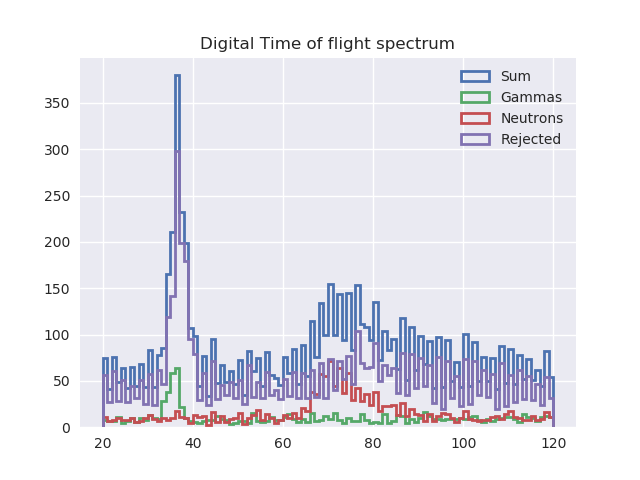
\includegraphics[width=0.8\textwidth]{DigitalResults/tof_psd.pdf}
        \caption{}
        \label{fig:tof_digi_cc}
    \end{subfigure}
	\begin{subfigure}[ht]{\textwidth}
		\centering
        \includegraphics[width=0.8\textwidth]{DigitalResults/CNNtof_psd.pdf}
        \caption{}
        \label{fig:tof_digi_cnn}
    \end{subfigure}
    \caption[Pulse shape parameters as function of time of flight, digital setup.]{Heatmaps of of pulseshape discrimination parameters as functions of time of flight plotted with logarithmic z-axis.}
    \label{fig:tof_cc_tof_cnn}
\end{figure}



\section{Misidentification}\label{sec:comp}


Another way to compare the performance of the PSD methods is by estimating the misclassification rate. This can be done by evaluating the time of flight spectrum in three different regions and comparing the relative number of neutron and gamma-ray labeled events. Ideally the number of gamma-rays identified per nanosecond channel in a background region, containing only random coincidences, should be the same as the number of gamma-rays identified in the neighborhood of the neutron time of flight peak. Likewise the number of neutrons identified at the gamma peak should correspond to the neutron background. The misclassification rate of gamma-rays and neutrons, 
M$_{\gamma}$ and M$_\textrm{n}$ respectively can be expressed as

\begin{equation}
	M_\gamma(R_\gamma) = \frac{N_{n}(R_\gamma)-\langle N_n(R_\gamma)\rangle}{N_{total}(R_\gamma)-\langle N_n(R_\gamma)\rangle}
\end{equation}

\begin{equation}
	M_n(R_n) = \frac{N_{\gamma}(R_n)-\langle N_\gamma(R_n)\rangle}{N_{total}(R_n)-\langle N_\gamma(R_n)\rangle},
\end{equation}
where N$_n$ and N$_\gamma$ are the number of neutrons and gamma-rays identified in region R and $\langle \textrm{N}_\textrm{n}\rangle$ and $\langle \textrm{N}_\gamma\rangle$ are the expected numbers found by normalizing the background rates to the width of R.

This definition of misclassification rate relies on the assumption that the choice of limits for each of the three regions does not seriously impact the results. It was found that as long as the peaks were contained in the region the misclassification rates in percent would change by at most $\pm$0.5\% for the digital setup and at most $\pm$1\% for the analog setup. The neutron peak limits were set to match the range of neutron energies 1.5-\SI{7}{\MeV} and the gamma peak neighborhood was selected as \SI{5}{\ns} on either side of the gamma-ray peak.

Figure~\ref{fig:tof_cc_cnn} shows the time of flight spectrum obtained with the analog setup filtered according to the charge comparison method, as well as the spectrum obtained from the digital setup, filtered by charge comparison and by the CNN. gamma-rays are colored blue, neutrons red and their intersection is purple. Ideally the intersection of the distributions should be flat, but if there is some systematic misclassification, then the intersection will rise up above the background level at the neutron and gamma peaks. This is an expression of the extent of misclassification of the given PSD implementation.

For the analog setup a high degree of contamination is evident in the form of the two purple peaks coinciding with the neutron and gamma peaks. This gives an estimated misclassification of 13\% for neutrons and 12\% for gamma-rays. From Fig.~\ref{fig:tof_ps_a} it was found that a number of the injected YAP start triggers remained even after cutting away events below \SI{0.8}{\MeV}, and that these landed at the gamma ToF but with very high PS values. These events may be part of the reason why there is nearly 12\% misclassification near the gamma-ray peak.

The digital setup provides a lower misclassification rate with the charge comparison method, at 10\% for neutrons and 3\% for gamma-rays. The much higher misclassification for neutrons imply that the model is biased towards gamma-rays.

The CNN approach reaches even better results with gamma-ray misclassification of 4\% and neutron misclassification rate of 5\%.
This is a significant improvement compared to the charge comparison method, and with the misclassification of nearly the same amount for both neutrons and gamma-rays the CNN method does not appear to have a strong bias towards either particle species.

The neutron background is found to be nearly the same by the analog and digital charge comparison methods, at 37\% and 38\% respectively. The CNN method finds a significantly higher background of neutron events at 45\%. This together with the high misclassification rates for the charge comparison methods hints at them being biased towards gamma-rays.

The correct fraction of events due to neutrons interacting in the NE213 is not trivial to determine. Although the radiation emitted by the source is approximately isotropic radiation scattered by the aquarium and walls of the room complicates matters. So to get a better idea of what fraction of neutrons to expect simulations are needed. It is however clear that the CNN distribution is better at reproducing a flat background of neutrons at the gamma peak and vice versa, than the digital and analog charge comparison methods, so it seems likely that 45\% is a better estimate.



\begin{figure}
    \centering
    \begin{subfigure}[bh]{\textwidth}
   	   	\centering
	    \includegraphics[width=0.85\textwidth]{AnalogResults/ToF_filt.pdf}
    	\caption{Time of flight spectrum filtered by a linear cut at PS = 0.259.}
    	\label{fig:ToF_filt_A}
   	\end{subfigure}
    \begin{subfigure}[bh]{\textwidth}
   	    \centering
        \includegraphics[width=0.85\textwidth]{DigitalResults/ToF_filt.pdf}
        \caption{Time of flight spectrum filtered by a linear cut at PS=0.222.}
        \label{fig:ToF_filt_D}
    \end{subfigure}
	\begin{subfigure}[bh]{\textwidth}
	    \centering
        \includegraphics[width=0.85\textwidth]{DigitalResults/CNNToF_filt.pdf}
        \caption{Time of flight spectrum filtered by a linear cut at prediction = 0.5.}
        \label{fig:ToF_filt_D_CNN}
    \end{subfigure}
	\caption[Misclassification of different PSD implementations.]{Misclassification of different PSD implementations.}
    \label{fig:tof_cc_cnn}
\end{figure}


\section{Fractional Energy Deposition}

The heatmap shown in Fig.~\ref{fig:tof_E_d} shows energy deposition in the NE213 detector as a function of time of flight. The gamma-ray distribution is constituted of gamma-rays that were produced in the deexcitation of $^\mathrm{12}$C (\SI{4.44}{MeV} gamma rays) or in deexcitation of $^\mathrm{234}$U (cascade of low energy gamma rays) as described in the chapter~\ref{ch:1}. From the distribution in the figure it seems that the low energy gamma-rays are particularly dominating in the gamma-flash.

The \SI{2.23}{MeV} gamma peak seen in the PSD and Energy spectra should not be visible in Fig.~\ref{fig:tof_E_d} as these gamma-rays are produced in an entirely different process by neutrons being absorbed by hydrogen nuclei. Strangely However, the figure shows a nearly continuous distribution of gamma-rays from 0 up to around \SI{4.5}{MeV}.

\begin{figure}[ht]
    \centering
        \includegraphics{DigitalResults/tof_E.pdf}
        \caption[Time of flight plotted against energy deposition.]{Time of flight plotted against energy deposition.}
    \label{fig:tof_E_d} 
\end{figure}

The neutron distribution shows a relation between time of flight and deposited energy. The slowest neutrons have a smaller spread in deposited energy, whereas the faster ones have a much wider spread. This is because the neutron in each elastic scattering can loose up to a certain fraction of it's total kinetic energy, as described by Eq.~\ref{eq:scat}. In NE213 the neutron primarily scatters against hydrogen nuclei. By Eq.~\ref{eq:scat} it is then possible for the neutron to deposit anywhere between 0 and 100\% of its energy, with 0\% implying the neutron missed the nucleus and 100\% implying a head on collision.

In Fig.~\ref{fig:N_E} this relation is highlighted. The top panel shows the ratio of deposited energy to neutron kinetic energy as a function of neutron energy. The red point represent the center of Gaussian functions fitted to the ratio of deposited to kinetic energy for narrow slices of neutron kinetic energies. the dotted line is the center point of the same type of fit covering all neutron energies. The ratio is nearly constant over the entire energy range, which suggests that the relation between deposited energy and neutron kinetic energy is approximately linear.

In fact the scintillation light output produced by an NE213 detector is expected to follow the following Eq.\cite{Scherzinger:2016}, Which approaches a linear shape at as neutron energies rise and the exponential term approaches unity:
\begin{equation}
	E_{deposited} = C\left(  0.83\cdot E_{neutron} - 2.82\cdot\left(  1 - e^{(-0.25\cdot E_{neutron}^{0.93})}  \right)  \right)
\end{equation}
The parameter C depends on the particular detector and can be found through fitting. In the bottom panel of Fig~\ref{fig:N_E} each red point represents the center of a Gaussian fitted to the deposited energies corresponding to a narrow slice of neutron energies. The value of C was found to be 0.794. The fact that the fit doesn't match the points so well at lower neutron energies may be due to the amplitude threshold particularly affects the low energy neutrons.

\begin{figure}[ht]
    \centering
        \includegraphics{DigitalResults/N_E.pdf}
        \caption[Neutron kinetic energy and deposited energy.]{Top: Ratio of deposited energy to neutron kinetic energy. Bottom: deposited energy as a function of neutron kinetic energy, along with fits.}
    \label{fig:N_E} 
\end{figure}



\end{document}